% Chapter 1

\chapter{Parabolic Problem} % Main chapter title

\label{Chapter2} % For referencing the chapter elsewhere, use \ref{Chapter1} 

\lhead{Chapter 2. \emph{Parabolic and 2D Problem}} % This is for the header on each page - perhaps a shortened title

%----------------------------------------------------------------------------------------

\section{Parabolic Problem}
We consider the convection-diffusion-reaction equation with the following conditions
\begin{align}
 & u_{t}-\epsilon u_{xx} + bu_{x} + cu = f \text{ for } (x,t) \in \Omega=(0,1)\\
 & u(x,0) = \phi(x)\\
 & u(0,t) = \alpha(t), u(1,t) = \beta(t)
\end{align}
The coefficients on the grid points are approximated as follows:
\begin{align*}
 b(x,t) \approx b_{j}^{n}, \hspace{5mm} c(x,t) \approx c_{j}^{n}, \hspace{5mm}f(x,t) \approx f_{j}^{n} \text{ for } x \in [x_{j-1},x_{j+1}],\hspace{2mm} t \in [t^{n},t^{n+1}]
\end{align*}
Thus the equation is now,
\begin{align*}
 u_t -\epsilon u_{xx} + b_{j}^{n} + c_{j}^{n} = f_{j}^{n} \text{ for } x \in [x_{j-1},x_{j+1}],\hspace{2mm} t \in [t^{n},t^{n+1}]
\end{align*}
For $c_{j}^{n}>0$, we let $v(x,t) = u(x,t)-f_{j}^{n}/c_{j}^{n}$. Then $v(x,t)$ satisfies
\begin{align*}
 v_t-\epsilon v_{xx} + b_{j}^{n} + c_{j}^{n}v = 0 \text{ for } x \in [x_{j-1},x_{j+1}],\hspace{2mm} t \in [t^{n},t^{n+1}]
\end{align*}
Let
\begin{align*}
 H_{3} = \{ w(x,t) | = w(x,t) = \beta_{0}e^{-c_{j}^{n}t}, \beta_{1}e^{\lambda_{+}x},\beta_{2}e^{\lambda_{-}x} \text{ for } \beta_{i} \in R     \}
\end{align*}
with
\begin{align*}
 \lambda_{\pm} = \frac{b_{j}^{n}}{2\epsilon} \pm \sqrt{\frac{(b_{j}^{n})^2}{4 \epsilon^2}+\frac{c_{j}^{n}}{\epsilon}}
\end{align*}
We use the following scheme
\begin{align*}
 v_{j}^{n+1} = \alpha_{1}v_{j-1}^{n}+\alpha_{2}v_{j}^{n}+\alpha_{3}v_{j+1}^{n}
\end{align*}
Substituting the basis functions in the above scheme we obtain

\begin{align}
 \alpha_{1}+\alpha_{2}+\alpha_{3} &= e^{-c_{j}^{n}\tau}\\
 \alpha_{1}e^{-\lambda_{+}h}+\alpha_{2}+\alpha_{3}e^{\lambda_{+}h} &= 1\\
 \alpha_{1}e^{-\lambda_{-}h}+\alpha_{2}+\alpha_{3}e^{\lambda_{-}h} &= 1
\end{align}

On solving the above system we get

\begin{align}
\alpha_{1} &= \frac{e^{-\lambda_{+}h}(1-e^{-c_{j}^{n}}\tau)}{(1-e^{-\lambda_{+}h})(1-e^{\lambda_{-}h})}\\
\alpha_{3} &= \frac{e^{\lambda_{-}h}(1-e^{-c_{j}^{n}}\tau)}{(1-e^{-\lambda_{+}h})(1-e^{\lambda_{-}h})}\\
\alpha_{2} &= e^{-c_{j}^{n} \tau}-\alpha_{1}-\alpha_{3}
\end{align}

On substituting the expressions in the scheme we have the following expression

\begin{align*}
 u_{j}^{n+1} = \alpha_{1}u_{j-1}^{n}+\alpha_{2}u_{j}^{n}+\alpha_{3}u_{j+1}^{n} + (1-e^{-c_{n}^{j}\tau})\frac{f_{j}^{n}}{c_{j}^{n}}
\end{align*}

\subsection{Stability criterion}
The stability criterion is given as
\begin{align*}
 \alpha_{1} + \alpha_{3} \leq \frac{1+e^{-c \tau}}{2}
\end{align*}
This scheme is claimed to have second order convergence.
\subsection{Example}
Consider the equation along with the given initial conditions and boundary conditions
\begin{align}
 \begin{split}
  &u_{t}-\epsilon u_{xx} + 2u_{x} + u = f(x,t)\\
  &f(x,t) = e^{2(x-1)/\epsilon}(2\cos(2t)+\sin(2t))+e^{(x-1)}(cos(t)-\epsilon \sin(t)+3\sin(t))
 \end{split} 
\end{align}
The analytical solution is given by
\begin{align}
 u(x,t) = e^{2(x-1)/\epsilon}sin(2t) + e^{(x-1)}sin(t)
\end{align}

The following plots and error estimates have been obtained on solving the above example using the tailored finite point method.\\

\begin{tabular}{|c|c|c|c|c|c|}
   \hline
   (h, $\tau$)  & (1/16,$2*10^{-5}$)  & (1/32,$2*10^{-5}$) & (1/64,$2*10^{-5}$) &(1/256,$2*10^{-5}$)\\
  \hline
  Error  & 0.00253  & 0.00064 & 0.00015 & 0.00003\\
  \hline
  Order & -  &  1.97  & 2.013 & 2.09\\
\hline
\end{tabular}

\clearpage

\begin{figure}[htbp]
	\centering
		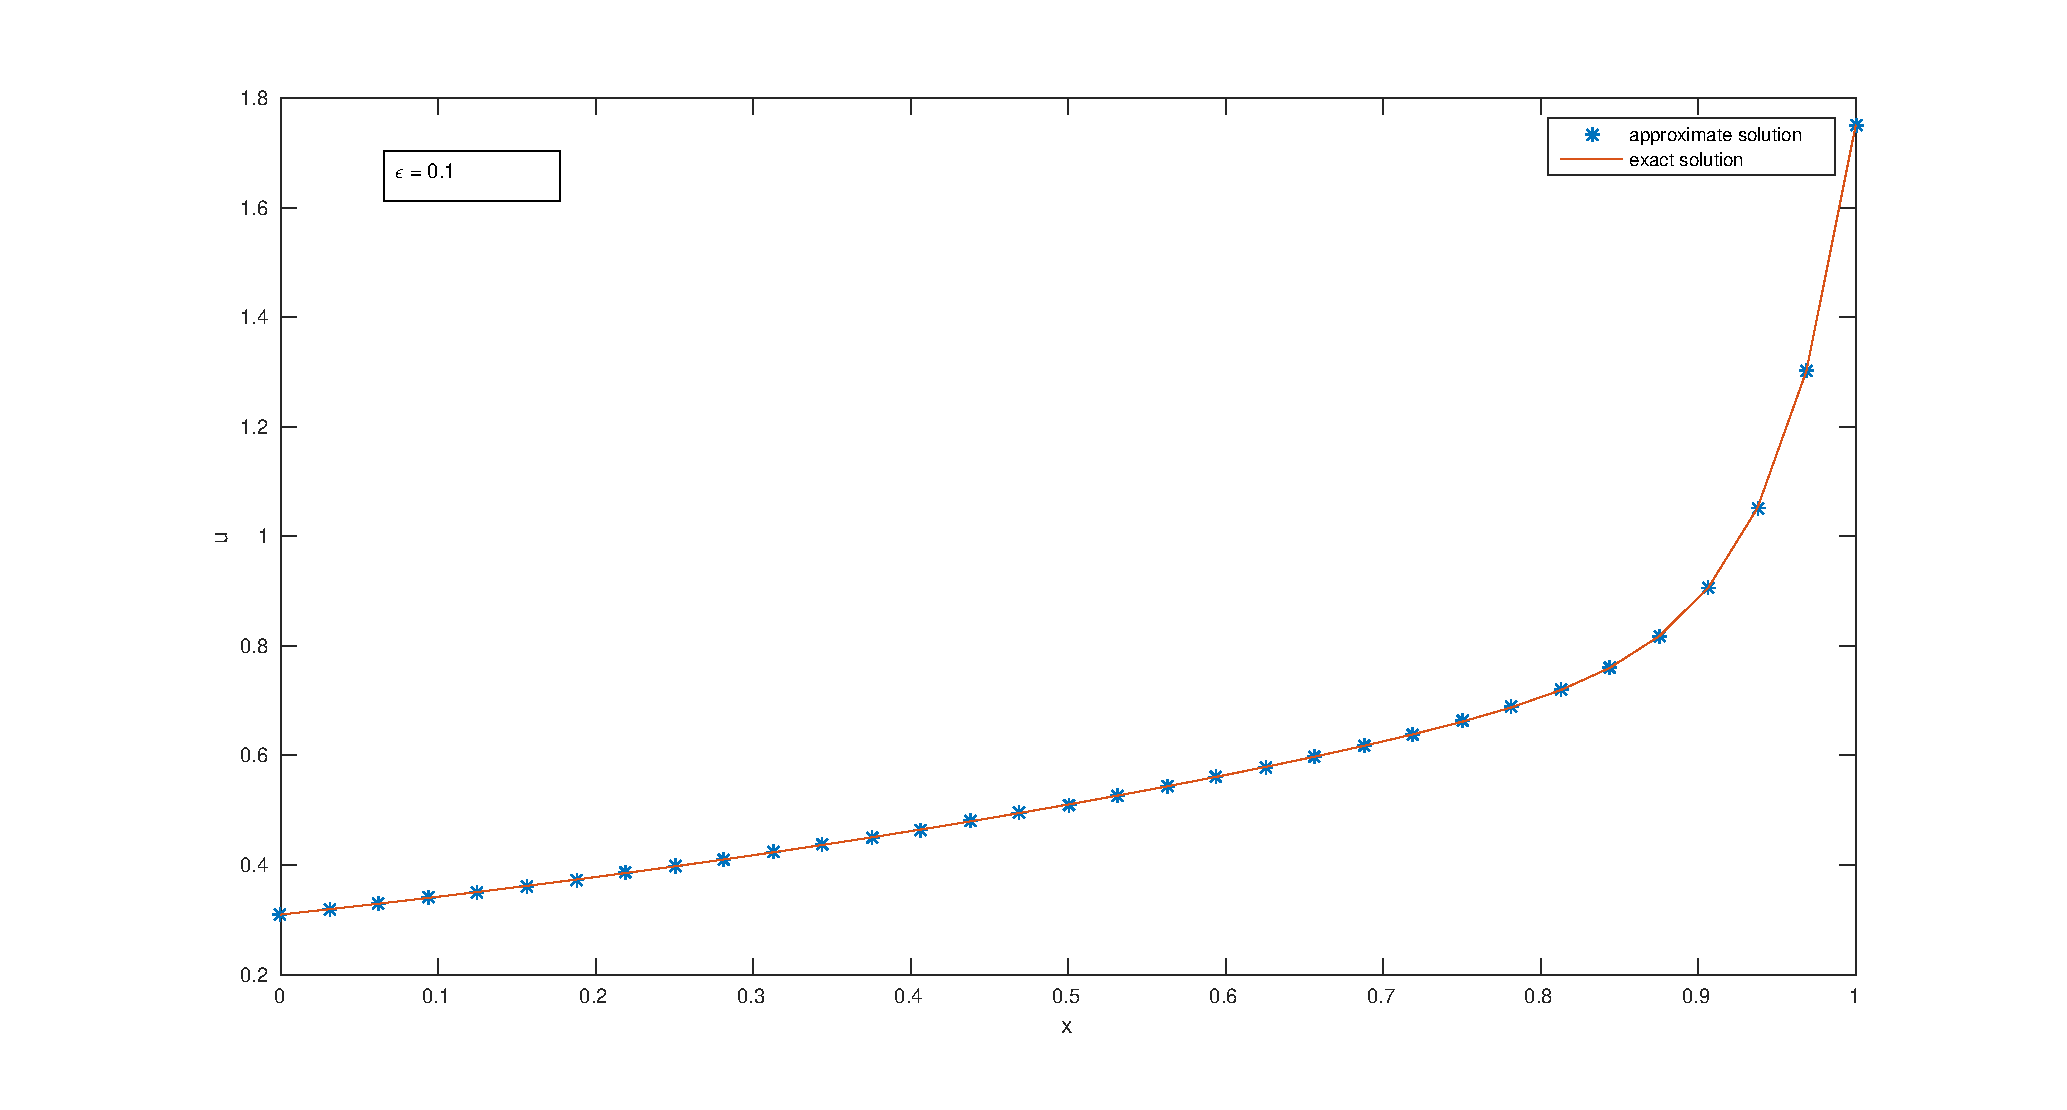
\includegraphics[height=8cm]{Figures/explicit5_2.eps}\\
		\rule{35em}{0.5pt}
	\caption[Parablic]{}
\end{figure}



